\documentclass{article}

\usepackage[margin=1in,left=1.5in,includefoot]{geometry}
\usepackage{graphicx}

\begin{document}

\begin{titlepage}
	\begin{center}
	\line(1,0){300}\\
	[0.25inc]
	\huge{\bfseries The Destribution and Nature of Agriculture in Uganda}\\
	[2mm]
	\line(1,0){200}\\
	[1.5cm]
	\end{center}

	\begin{flushright}
	\textsc{\large MUWONGE TIMOTHY.\\
	\#14/U/23570/Eve \\
	\# 214023412\\
	May 14, 2017\\}
	\end{flushright}
\end{titlepage}
\cleardoublepage

\tableofcontents
\thispagestyle{empty}
\cleardoublepage
\pagenumbering{arabic}
\setcounter{page}{1}

\section{Abstruct}

This report contains an abstruction of the agricultural sector of uganda where by samples of the farms in uganda where taken and evaluated to see where the agricutual sector lies in today's uganda.

This report contains detailed information of the farms and there destribution partern in Uganda

The information is taken from the some of the farms in my Region

Further more, after the data collection , the information of the facilities is sent to the Open Data Kit (ODK) aggregate server. This report explains all about the data and the findings
\section{Introduction}

Being a landlocked equatorial region country, Uganda experiences reliable rainfall, reliable sun shine, possesses fertile soils, has a favorable climate with no tornados and snow, has a relatively flat relief, and also gifted with rich lakes and rivers most of which are none seasonal in nature. 

All these features have been a stepping stone for the growth of agriculture in Uganda since they all support agricultural activities in such a way that they provide the basic requirement necessary for farming.

\section{Background}

Uganda is regarded as an agriculture-based economy and a food basket in the Eastern 
African region, given its ability to produce a variety of foods and in large quantities.    It 
comprises of the food and cash crops production,  livestock,  forestry  and  fishing  subsectors.    These  sub-sectors  contributed  62,  8,  17  and  13  percent  respectively  to 
agricultural  Gross  Domestic  Product  (GDP)  in  2011/12.    Agriculture  is  considered  an 
important  sector  that  contributed  23.7  percent  to  GDP  (at  current  prices)  in  2011/12. 
According to the  UCA  2008/9, there were approximately 3.95 million small and medium 
agricultural  households  with  a  population  of  19.3m  persons  (60\%  of  the  Uganda’s 
population) these produced the bulk (over 95 percent) of the food and cash crops.

The  agriculture  sector,  which  is  mainly  subsistence,  employs  the  largest  proportion  of 
Uganda’s work force. During the  Population and Housing Census (PHC)  2002,  about  73 
percent  (81  percent  female  and  67  percent  males)  of  the  work  force  was  employed  in 
agriculture,  making it the dominant  economic activity at that time.    The sector  remains  a
major  employer  to  date,  with  70  percent  and  66  percent  of  the  working  population 
engaged in agriculture during 2009/10 and 2010/11 respectively.  The sector is crucial for 
general  growth  of the  economy  (providing  inputs  into  the  industrial  sector)  and  poverty 
reduction especially among the rural poor for whom it provides employment.

After having gone through all the alleged current information about the agricultural sector in Uganda currently, I have chosen to investigate on the extent to which these allegations are true in otherward, to carry out a survey to determine the distribution of agriculture in Uganda


\section{Aim and Objectives}\label{sec:aimsandobjectives}
\subsection{Aim or general objective}
Aim:  To develop a fully populated database having all details about the farms in Uganda today and where they a located.

\subsection{Specific Objectives}

To move throughout the whole of Uganda identifying the Health facilities.

To find out the details needed from a farm in cases when a government is making a budget.

To design the database (physical and logical appearance).

To implement the design into a system.

To enter data into the database.

To test and validate the data.

\section{Methodology}

I visted agricultural gardens one at a time and at these farms ,I made interviews to the personals in charge ie Managers, and farmers with the aim of finding out what was carried out in the farm and how it was carried out .

The information details got include ; Photo of the farm, GPS cordinates, type of crops or animals , type of farming, size of the farm and the number of employees at the farm .\\

{\bfseries Data is collected using the ODK collect android app as shown below }\\ \\

\graphicspath{{farm/}}
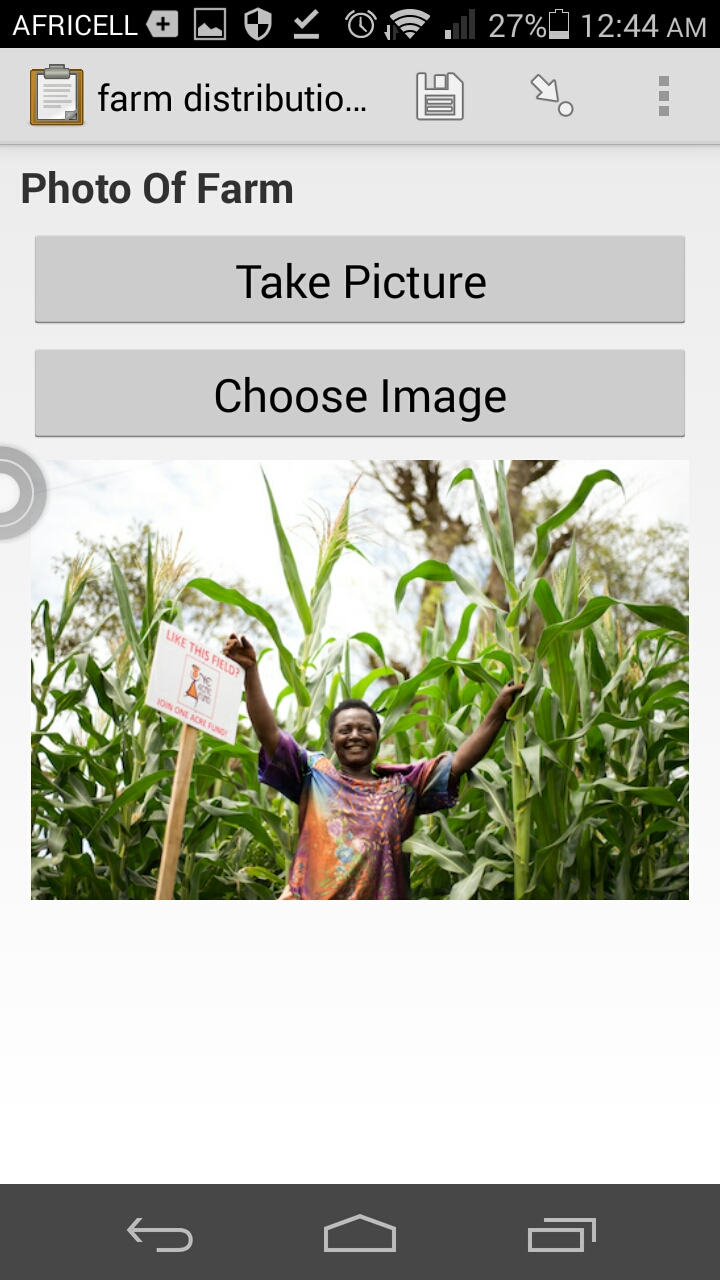
\includegraphics[width = 5cm , height = 8cm ]{1}
\graphicspath{{farm/}}
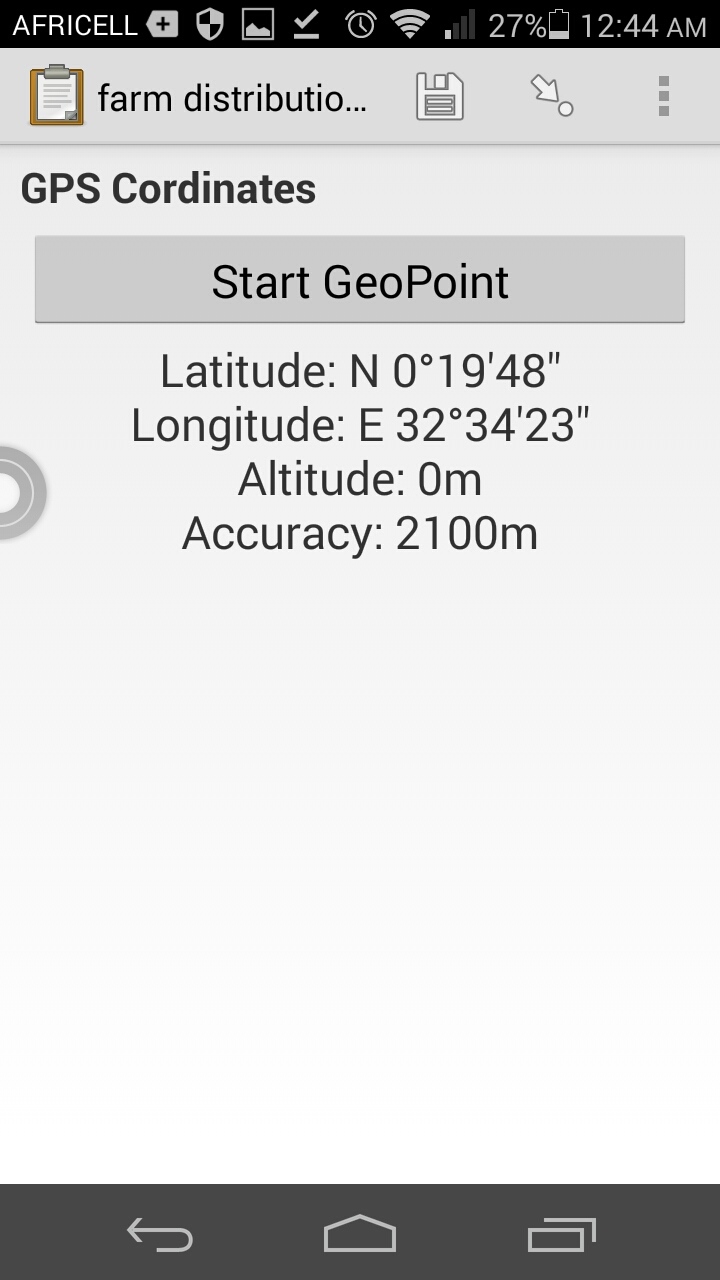
\includegraphics[width = 5cm , height = 8cm ]{11}
\graphicspath{{farm/}}
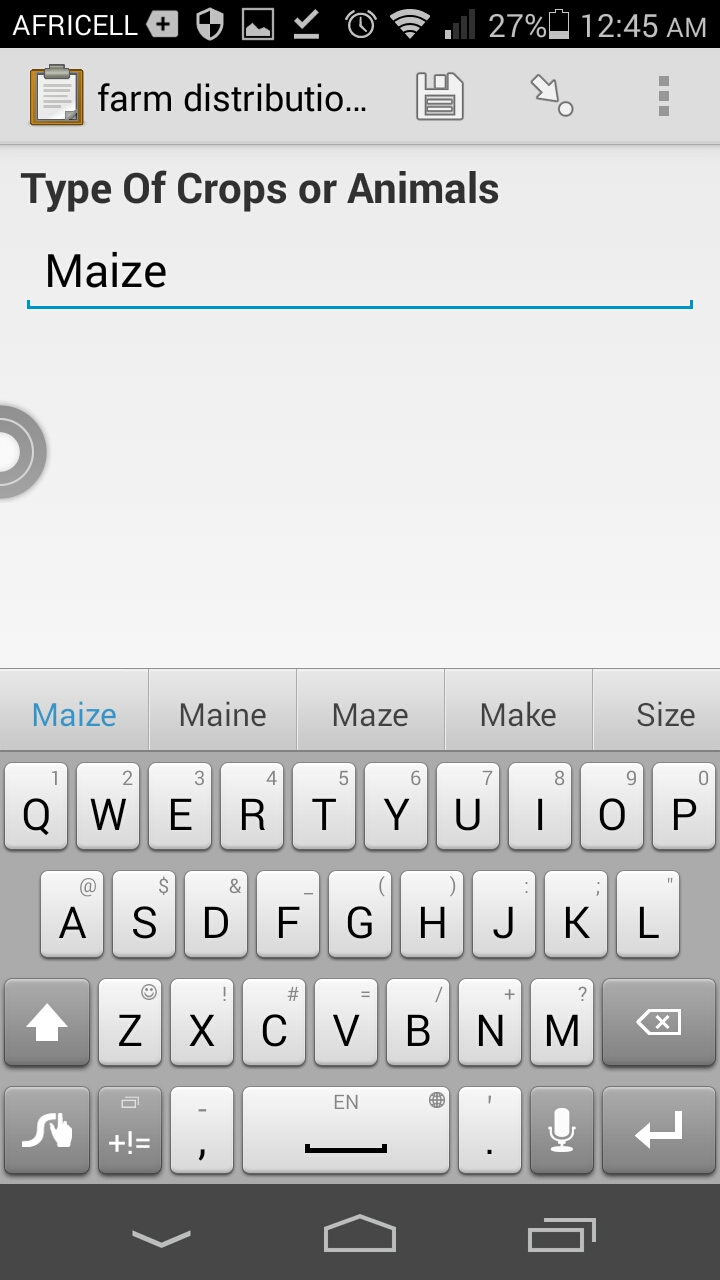
\includegraphics[width = 5cm , height = 8cm ]{111}
\graphicspath{{farm/}}
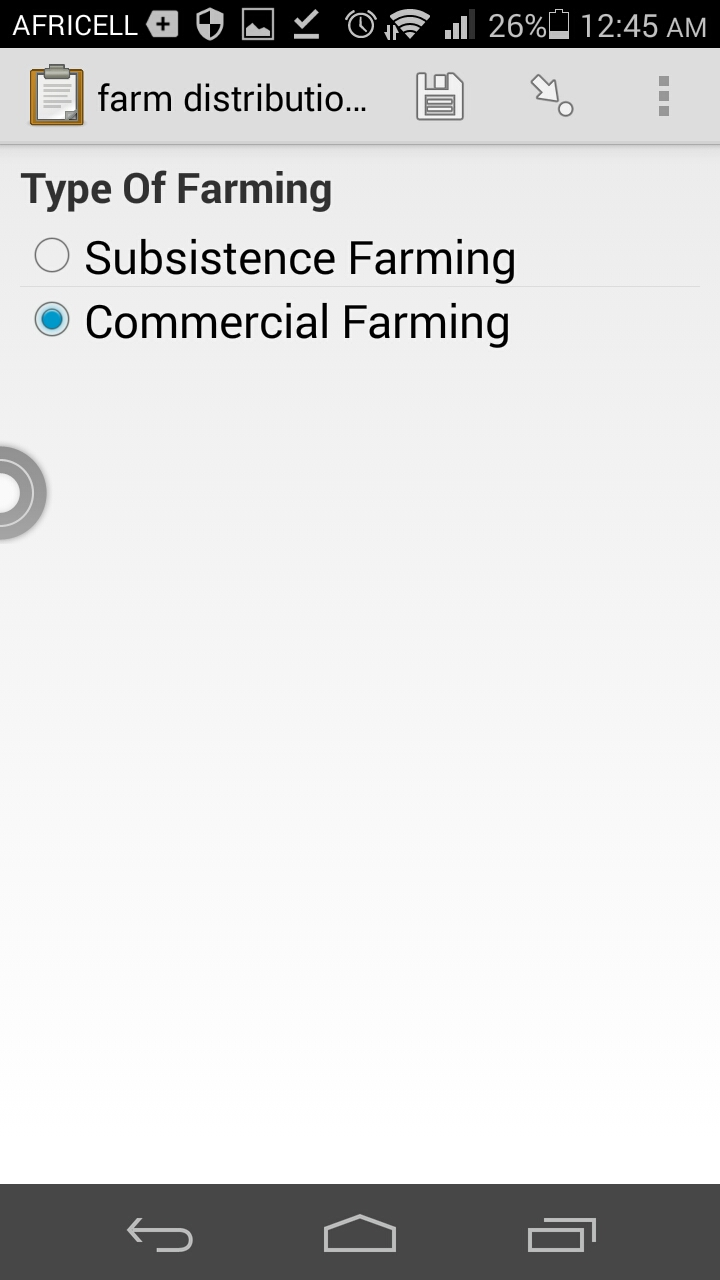
\includegraphics[width = 5cm , height = 8cm ]{1111}
\graphicspath{{farm/}}
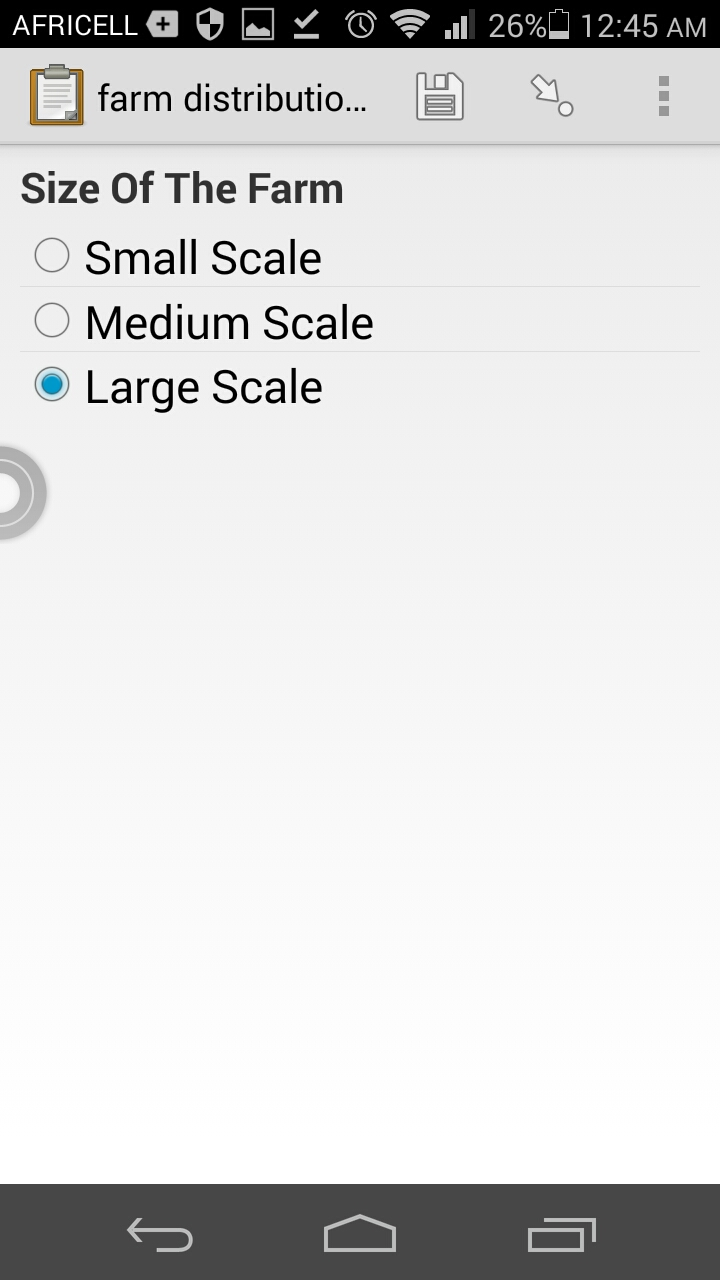
\includegraphics[width = 5cm , height = 8cm ]{11111}
\graphicspath{{farm/}}
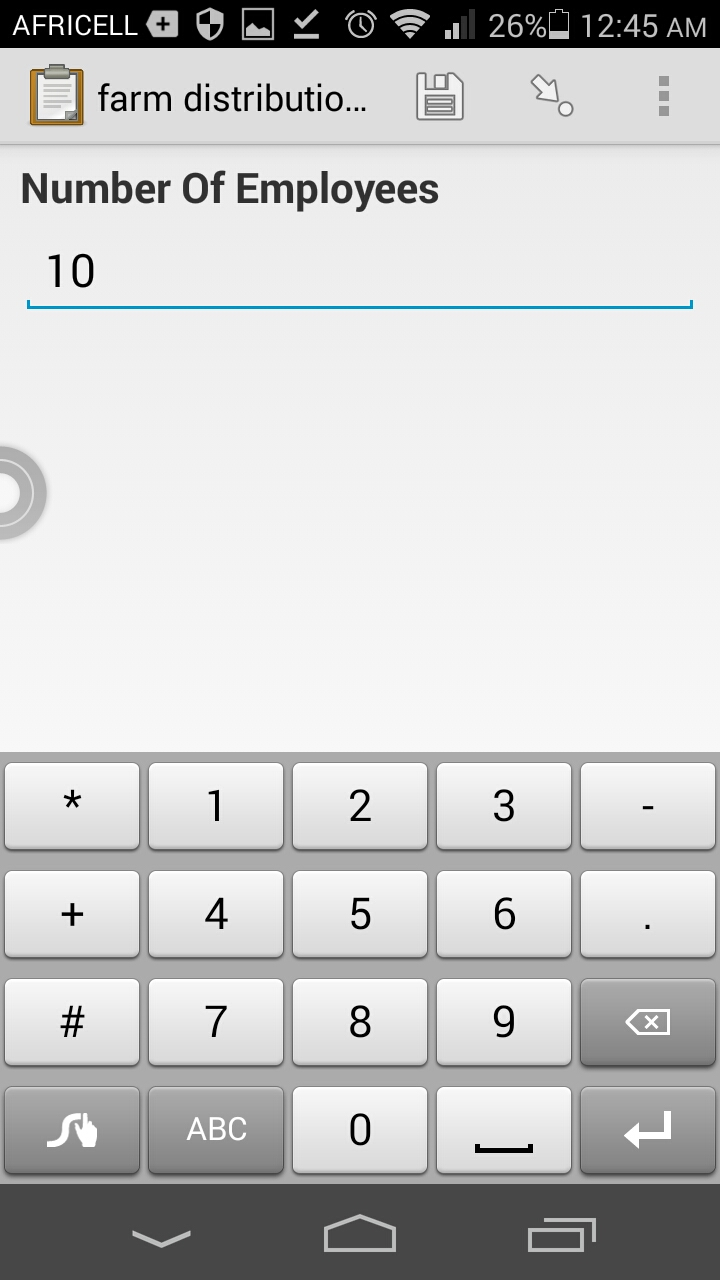
\includegraphics[width = 5cm , height = 8cm ]{111111}


\section{Data Analysis}

{\bfseries Data is The data on the ODK aggregate server is as shown below }\\
\graphicspath{{farm/}}
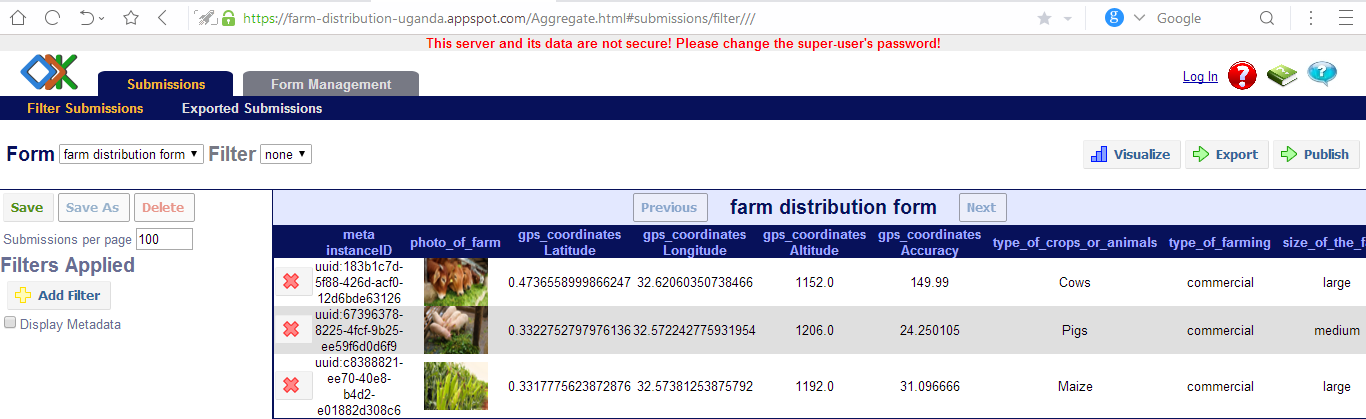
\includegraphics[width = 15cm , height = 5cm ]{farm}

\section{Conclusion}
Finally , The farms in uganda are basically on a small scale and very few of these are on large scale and because of this, there are a few people that are being employed in agriculture as a main source of income

These farms are largely located in the rural paets of uganda with very few of them being found in urban areas

In Uganda agriculture is majorly subsitance in nature where by most of the people practising farming do it for food and not money incomes

\section{References}


\end{document}